\begin{center}
	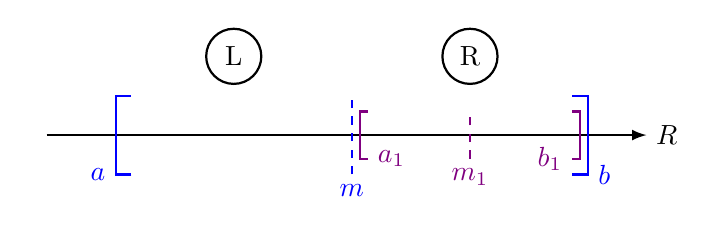
\begin{tikzpicture}
	[
		scale=1.0,
		>=latex,
		whitecircle/.style={circle, draw=black, fill=white, thick, minimum size=0.7cm},
	]

        % nodes
        \node               at (0, 0)   (O) {};             % Ursprung
        \node               at (8, 0)   (H) {$\mathbb{R}$}; % Pfeil-Ende
        \node[whitecircle]  at (2.5, 1) (L) {L};
        \node[whitecircle]  at (5.5, 1) (R) {R};
        
        % lines
        \draw[->, thick]            (O) -- (H);

        \draw[thick, blue]          (1.2, -0.5) -- (1, -0.5) node[left] (a) {$a$} -- (1, 0.5) -- (1.2, 0.5);
        \draw[thick, blue]          (6.8, -0.5) -- (7, -0.5) node[right] (b) {$b$} -- (7, 0.5) -- (6.8, 0.5);
        \draw[thick, blue, dashed]  (4, -0.5) node[below] (m) {$m$} -- (4, 0.5);

        \draw[thick, violet]        (4.2, -0.3) node[right] (a1) {$a_1$} -- (4.1, -0.3) -- (4.1, 0.3) -- (4.2, 0.3);
        \draw[thick, violet]        (6.8, -0.3) node[left] (b1) {$b_1$}-- (6.9, -0.3)  -- (6.9, 0.3) -- (6.8, 0.3);
        \draw[thick, violet, dashed](5.5, -0.3) node[below] (m1) {$m_1$} -- (5.5, 0.3);
    \end{tikzpicture}
\end{center}